\chapter{Проектирование базы данных приложения}

        В данной главе будет представлен процесс проектирования базы данных %
        веб-приложения для составления графика лечения на основании рекомендаций %
        врача.
        
    \section{Потенциальные объекты системы}
        В процессе анализа предметной области были выделены следующие примерные %
        бизнес-сущности, которые должны быть отображены в базе данных:

        \begin{itemize}
            \item Доктор;
            \item Пациент;
            \item Менеджер;
            \item Прием лекарств;
            \item Прием врача;
            \item Лекарственное средство;
            \item Рекомендации;
            \item Отзыв;
        \end{itemize}

    \section{Определение атрибутов и первичных ключей}

        Для оптимизации работы веб-приложения, было принято решение о %
        денормализации базы данных, объединив объекты системы в сущность "Пользователь". %
        Для реализации контроля доступа внутри системы будет введен атрибут роли, %
        который будет ограничивать доступ к изменению и получения данных из системы. %

        В таблице \ref{user-attrs-table} представлены атрибуты сущности "Пользователь".

        \begin{table}[H]
            \caption{Описание атрибутов сущности "Пользователь".}
            \label{user-attrs-table}
            \resizebox{\columnwidth}{!}{%
            \begin{tabular}{|p{0.225\linewidth}|p{0.3\linewidth}|p{0.2\linewidth}|p{0.2\linewidth}|}
            \hline
            Название атрибута & Обязательный/не обязательный (*/o) & Уникальный идентификатор (\#) & Тип для логической модели \\
            \hline
            idUser & * & \# & Числовой \\
            \hline
            email & * & (\#) & Символьный \\
            \hline
            role & * & & Символьный \\
            \hline
            firstName & * & & Символьный \\
            \hline
            secondName & * & & Символьный \\
            \hline
            lastName & & & Символьный \\
            \hline
            phoneNumber & & & Символьный \\
            \hline
            idTelegram & & & Числовой \\
            \hline
            idLicense & & & Символьный \\
            \hline
            isConfirmed & & & Логический \\
            \hline
            \end{tabular}%
            }
        \end{table}

        Поле "idTelegram"\ необходимо для авторации и рассылки уведомлений через %
        телеграмм-бота, который будет напоминать врачам и пользователям о изменении их %
        лечебного плана и о приеме необходимых лекарственных препаратов. 

        Поля "idLicense"\ и "isConfirmed"\ относятся к роли врача. "idLicense"\ %
        относиться к номеру идентифицирующему документ об образовании врача. %
        Поле "isConfirmed"\ показывает был ли допущен доктор к работе с пациентами после %
        проверки документов менеджером. 

    \newpage

    Взаимодействие между пациентом и доктором реализуется при помощи сущности пересечения, %
    которая показывает какие врачи производят наблюдения и рекомендации по лечебному плану для %
    определенного пользователя.

    В таблице \ref{patient-doctor-table} представлены атрибуты сущности пересечения между %
    ролями системы "Пациент"\ и "Доктор".
    \newline
    \begin{table}[H]
        \caption{Описание атрибутов сущности пересечения ролей  "Пациент"\ и "Доктор".}
        \label{patient-doctor-table}
        \resizebox{\columnwidth}{!}{%
        \begin{tabular}{|p{0.225\linewidth}|p{0.3\linewidth}|p{0.2\linewidth}|p{0.2\linewidth}|}
        \hline
        Название атрибута & Обязательный/не обязательный (*/o) & Уникальный идентификатор (\#) & Тип для логической модели \\
        \hline
        idUser & * & \# & Числовой \\
        \hline
        idDoctor & * & \# & Числовой \\ 
        \hline
        \end{tabular}%
        }
    \end{table}

    Для реализации уведомлений, была выделена сущность "Прием лекарств". %
    Данная сущность дожна хранить в себе атрибуты, для реализации следующих видов приема:
    
    \begin{itemize}
        \item Прием только один день;
        \item Ежедневный прием;
        \item Прием каждые X дней;
        \item Прием по конкретным датам;
        \item Цикл приема из X дней и Y дней пропуска; 
        \item Прием через определенный промежуток времени;
    \end{itemize}

    Также необходимо хранить время приема в течении дня для повышения %
    эффективности лечения.

    В таблице \ref{pills-table} представлены атрибуты сущности "Прием лекарств".
    \newline

    \begin{table}[H]
        \caption{Описание атрибутов сущности "Прием лекарств".}
        \label{pills-table}
        \resizebox{\columnwidth}{!}{%
        \begin{tabular}{|p{0.225\linewidth}|p{0.3\linewidth}|p{0.2\linewidth}|p{0.2\linewidth}|}
        \hline
        Название атрибута & Обязательный/не обязательный (*/o) & Уникальный идентификатор (\#) & Тип для логической модели \\
        \hline
        idPill & * & \# & Числовой \\
        \hline
        idUser & * &  & Числовой \\
        \hline
        type & * & & Символьный \\
        \hline
        name & * & & Символьный \\
        \hline
        form & & & Символьный \\
        \hline
        note & & & Симовльный \\
        \hline
        startDate & * & & Даты и времени \\
        \hline
        endDate & & & Даты и времени \\
        \hline
        time & & & Временной \\
        \hline
        days & & & Дата \\
        \hline
        deltaTakeDays & & & Числовой \\
        \hline
        deltaPassDays & & & Числовой \\
        \hline
        timeDelta & & & Временной \\
        \hline
        lastNotify & & & Даты и времени \\ 
        \hline
        \end{tabular}%
        }
    \end{table}
    
    Для отслеживание удовлетворенности пользвателей в услугах выбранного лечащего %
    врача была введена сущность "Отзыв". Данная сущность предназначена для администрирования %
    площадки менеджером и отслеживании качества предоставляемых докторами услуг. %
    Атрибуты сущности "Отзыв"\ представлены в таблице \ref{comment-table}

    \begin{table}[H]
        \caption{Описание атрибутов сущности "Отзыв".}
        \label{comment-table}
        \resizebox{\columnwidth}{!}{%
        \begin{tabular}{|p{0.225\linewidth}|p{0.3\linewidth}|p{0.2\linewidth}|p{0.2\linewidth}|}
        \hline
        Название атрибута & Обязательный/не обязательный (*/o) & Уникальный идентификатор (\#) & Тип для логической модели \\
        \hline
        idComment & * & \# & Числовой \\
        \hline
        idPatient & * &  & Числовой \\
        \hline
        idDoctor & * & & Числовой \\
        \hline
        rate & * & & Числовой \\
        \hline
        review & & & Символьный \\
        \hline

        \end{tabular}%
        }
    \end{table}

    Для эффективного процесса лечения также необходимы своевременное посещение %
    лечащего врача. Для этого в системе необходимо хранить информацию о плановых посещениях, %
    которые представлены в сущности "Прем врача". В таблице \ref{visit-table} %
    представлены атрибуты сущности "Прием врача".

    \begin{table}[H]
        \caption{Описание атрибутов сущности "Прием врача".}
        \label{visit-table}
        \resizebox{\columnwidth}{!}{%
        \begin{tabular}{|p{0.225\linewidth}|p{0.3\linewidth}|p{0.2\linewidth}|p{0.2\linewidth}|}
        \hline
        Название атрибута & Обязательный/не обязательный (*/o) & Уникальный идентификатор (\#) & Тип для логической модели \\
        \hline
        idVisit & * & \# & Числовой \\
        \hline
        idPatient & * &  & Числовой \\
        \hline
        idDoctor & & & Числовой \\
        \hline
        appointmentTime & * & & Даты и времени \\
        \hline
        note & & & Символьный \\
        \hline
        \end{tabular}%
        }
    \end{table}
    
    Для предоставления комфортного пользования сервисом были выделены справочные сущности, %
    которые позволяют пользователю ознакомиться с препаратами и предоставить поддержку советами %
    о правильном лечении.

    Сущность "Лекарственное средство"\ является справочной сущностью возможных %
    лекартсвенных препаратов. Аттрибуты данной сущности представлены в %
    таблице \ref{pills-type-table}

    \begin{table}[H]
        \caption{Описание атрибутов сущности "Лекарственное средство".}
        \label{pills-type-table}
        \resizebox{\columnwidth}{!}{%
        \begin{tabular}{|p{0.225\linewidth}|p{0.3\linewidth}|p{0.2\linewidth}|p{0.2\linewidth}|}
        \hline
        Название атрибута & Обязательный/не обязательный (*/o) & Уникальный идентификатор (\#) & Тип для логической модели \\
        \hline
        idPillType & * & \# & Числовой \\
        \hline
        name & * &  & Символьный \\
        \hline
        dose & * & & Числовой \\
        \hline
        form & * & & Символьный \\
        \hline
        description & & & Символьный \\
        \hline
        \end{tabular}%
        }
    \end{table}

    Сущность "Совет"\ является справочной сущностью, которая должна помочь пользователю %
    придерживаться эффективного плана лечения. Атрибуты сущности "Совет"\ представлены в %
    таблице \ref{tips-table}.
    
    \begin{table}[H]
        \caption{Описание атрибутов сущности "Совет".}
        \label{tips-table}
        \resizebox{\columnwidth}{!}{%
        \begin{tabular}{|p{0.225\linewidth}|p{0.3\linewidth}|p{0.2\linewidth}|p{0.2\linewidth}|}
        \hline
        Название атрибута & Обязательный/не обязательный (*/o) & Уникальный идентификатор (\#) & Тип для логической модели \\
        \hline
        idTips & * & \# & Числовой \\
        \hline
        title & * &  & Символьный \\
        \hline
        content & * & & Символьный \\
        \hline
        \end{tabular}%
        }
    \end{table}

    \section{Логическое проектирование базы данных}
        Логическое проектирование базы данных веб-прилоежения было произведено %
        при помощи программы "PgAdmin" \cite{pg-admin}. Данный комплекс программного обеспечения %
        является обширным инструментом для логического проектирования и %
        администрирования баз данных. Оно предоставляет возможность %
        создания ERD (Entity-Relationship Diagram) диаграмм, которые %
        представляют структуру базы данных и связи между ее элементами.
        "PgAdmin"\ также позволяет конвертировать ERD диаграммы в %
        SQL-скрипты, которые можно использовать для создания таблиц в %
        базе данных. Это значительно упрощает процесс разработки. %
        Результат преобразования сущностей в ERD диаграму изображен на рисунке \ref{erd_diagram}.

        \newpage
        \begin{landscape}
            \begin{figure}[H]%current location
                \centering
                \scalebox{0.42}{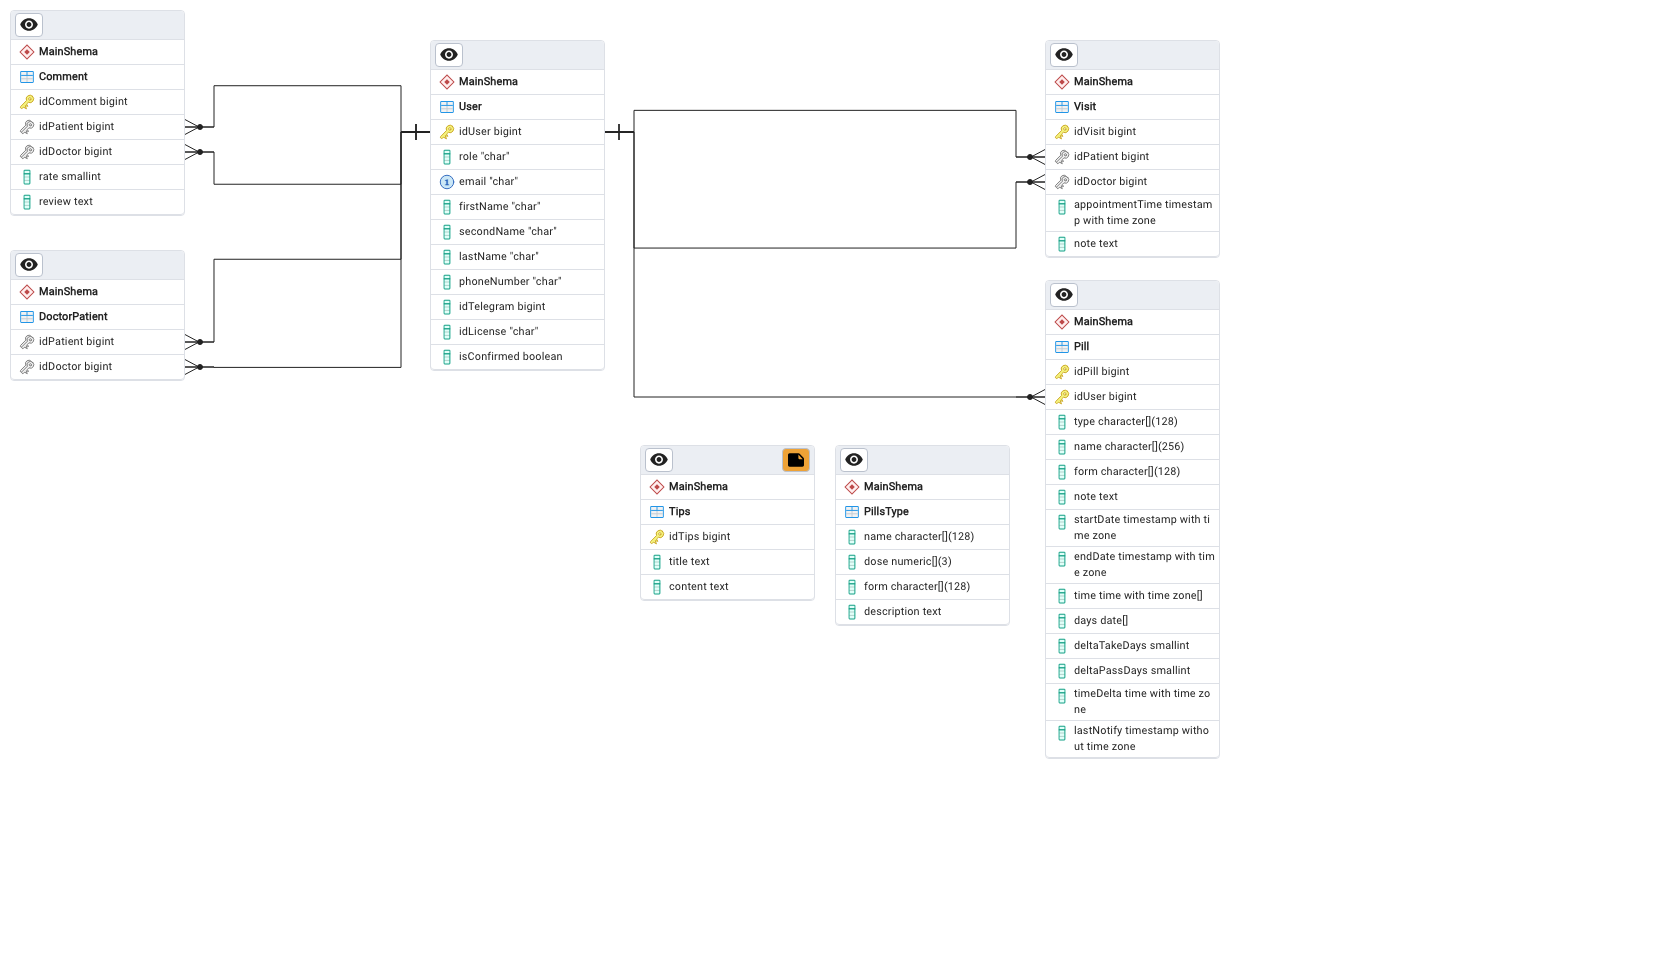
\includegraphics{pics/database/ERR-diagram.png}}
                \caption{ERD диаграмма базы данных.} \label{erd_diagram}
            \end{figure} 

        \end{landscape}